\chapter{Power Cycle Modeling Results}\label{ch:power_cycle_results}

\section{Reactor Mass Modeling Results}
The results of the reactor mass model are hard to analyze outside the context of
the overall power cycle optimization. In the most general sense, the reactor
mass model can be described as:

\begin{equation}
    m_{reactor} = f(\dot{m}, T_{in}, T_{out}, P_{in}, P_{out})
\end{equation}

The reactor is dependent on flow conditions, and configuration. Further
complicating the analysis, the flow conditions are coupled by the power cycle
efficiency.

\section{Reactor Response to Flow Inputs}

\subsection{Mass Flow Rate}
The mass flow rate through the core is dictated by the power cycle model. It is
the free variable used by the power cycle model to meet the required 40 kWe
output of the system. Increasing the mass flow rate improves the heat transfer
coefficient from the fuel to the coolant. Reactors with higher mass flow rates
have less resistance to convection and better cooling. While the mass flow rate
helps heat transfer in the reactor, it is also used to adjust power output. For
a fixed coolant temperature rise, increasing the mass flow rate increases the
required thermal output of the reactor. Increasing the output of the core always
increases the mass. Mass flow rate is a tradeoff between heat transfer
performance and required thermal power.

\subsection{Coolant Temperature}
Bulk coolant temperatures were used to calculate coolant properties and the
temperature drop from the fuel to coolant. Increasing the coolant temperture
decreases the temperture drop. This decrease in $\delta$T reduces the
coolability of the core, requiring a larger core volume to deliver the same
thermal power. While increasing coolant temperature reduces the thermal power
density of the reactor, it also improves the efficiency of the power cycle. A
more efficient cycle requires a smaller thermal input to generate a fixed amount
of electrical power.

\subsection{Coolant Pressure}
Bulk coolant pressures were used to calculate coolant properties. Pressure also
impacts the thickness of the pressure vessel. Higher pressure systems require a
thicker pressure vessel for containment.

\subsection{Thermal Power}
During the mass model development, reactor response to thermal power was the
metric to analyze changes in the model. The reactor mass is most strongly
dependent on thermal power. Core power density limits require larger reactor
masses for higher powers. A fixed coolant flow rate of 1 [kg/s] was used to test
the mass model. As mentioned previously, this is not a realistic test for the
reactor response since the mass flow rate of the coolant tends to increase with
increasing thermal power. Nevertheless, thermal power for fixed flow inputs was
used to test the mass model outside the context of the power cycle model. Figure
\ref{fig:mass_vs_q_uo2_co2} shows the reactor mass dependence on the power
cycle.

\begin{figure}[h]
    \centering
    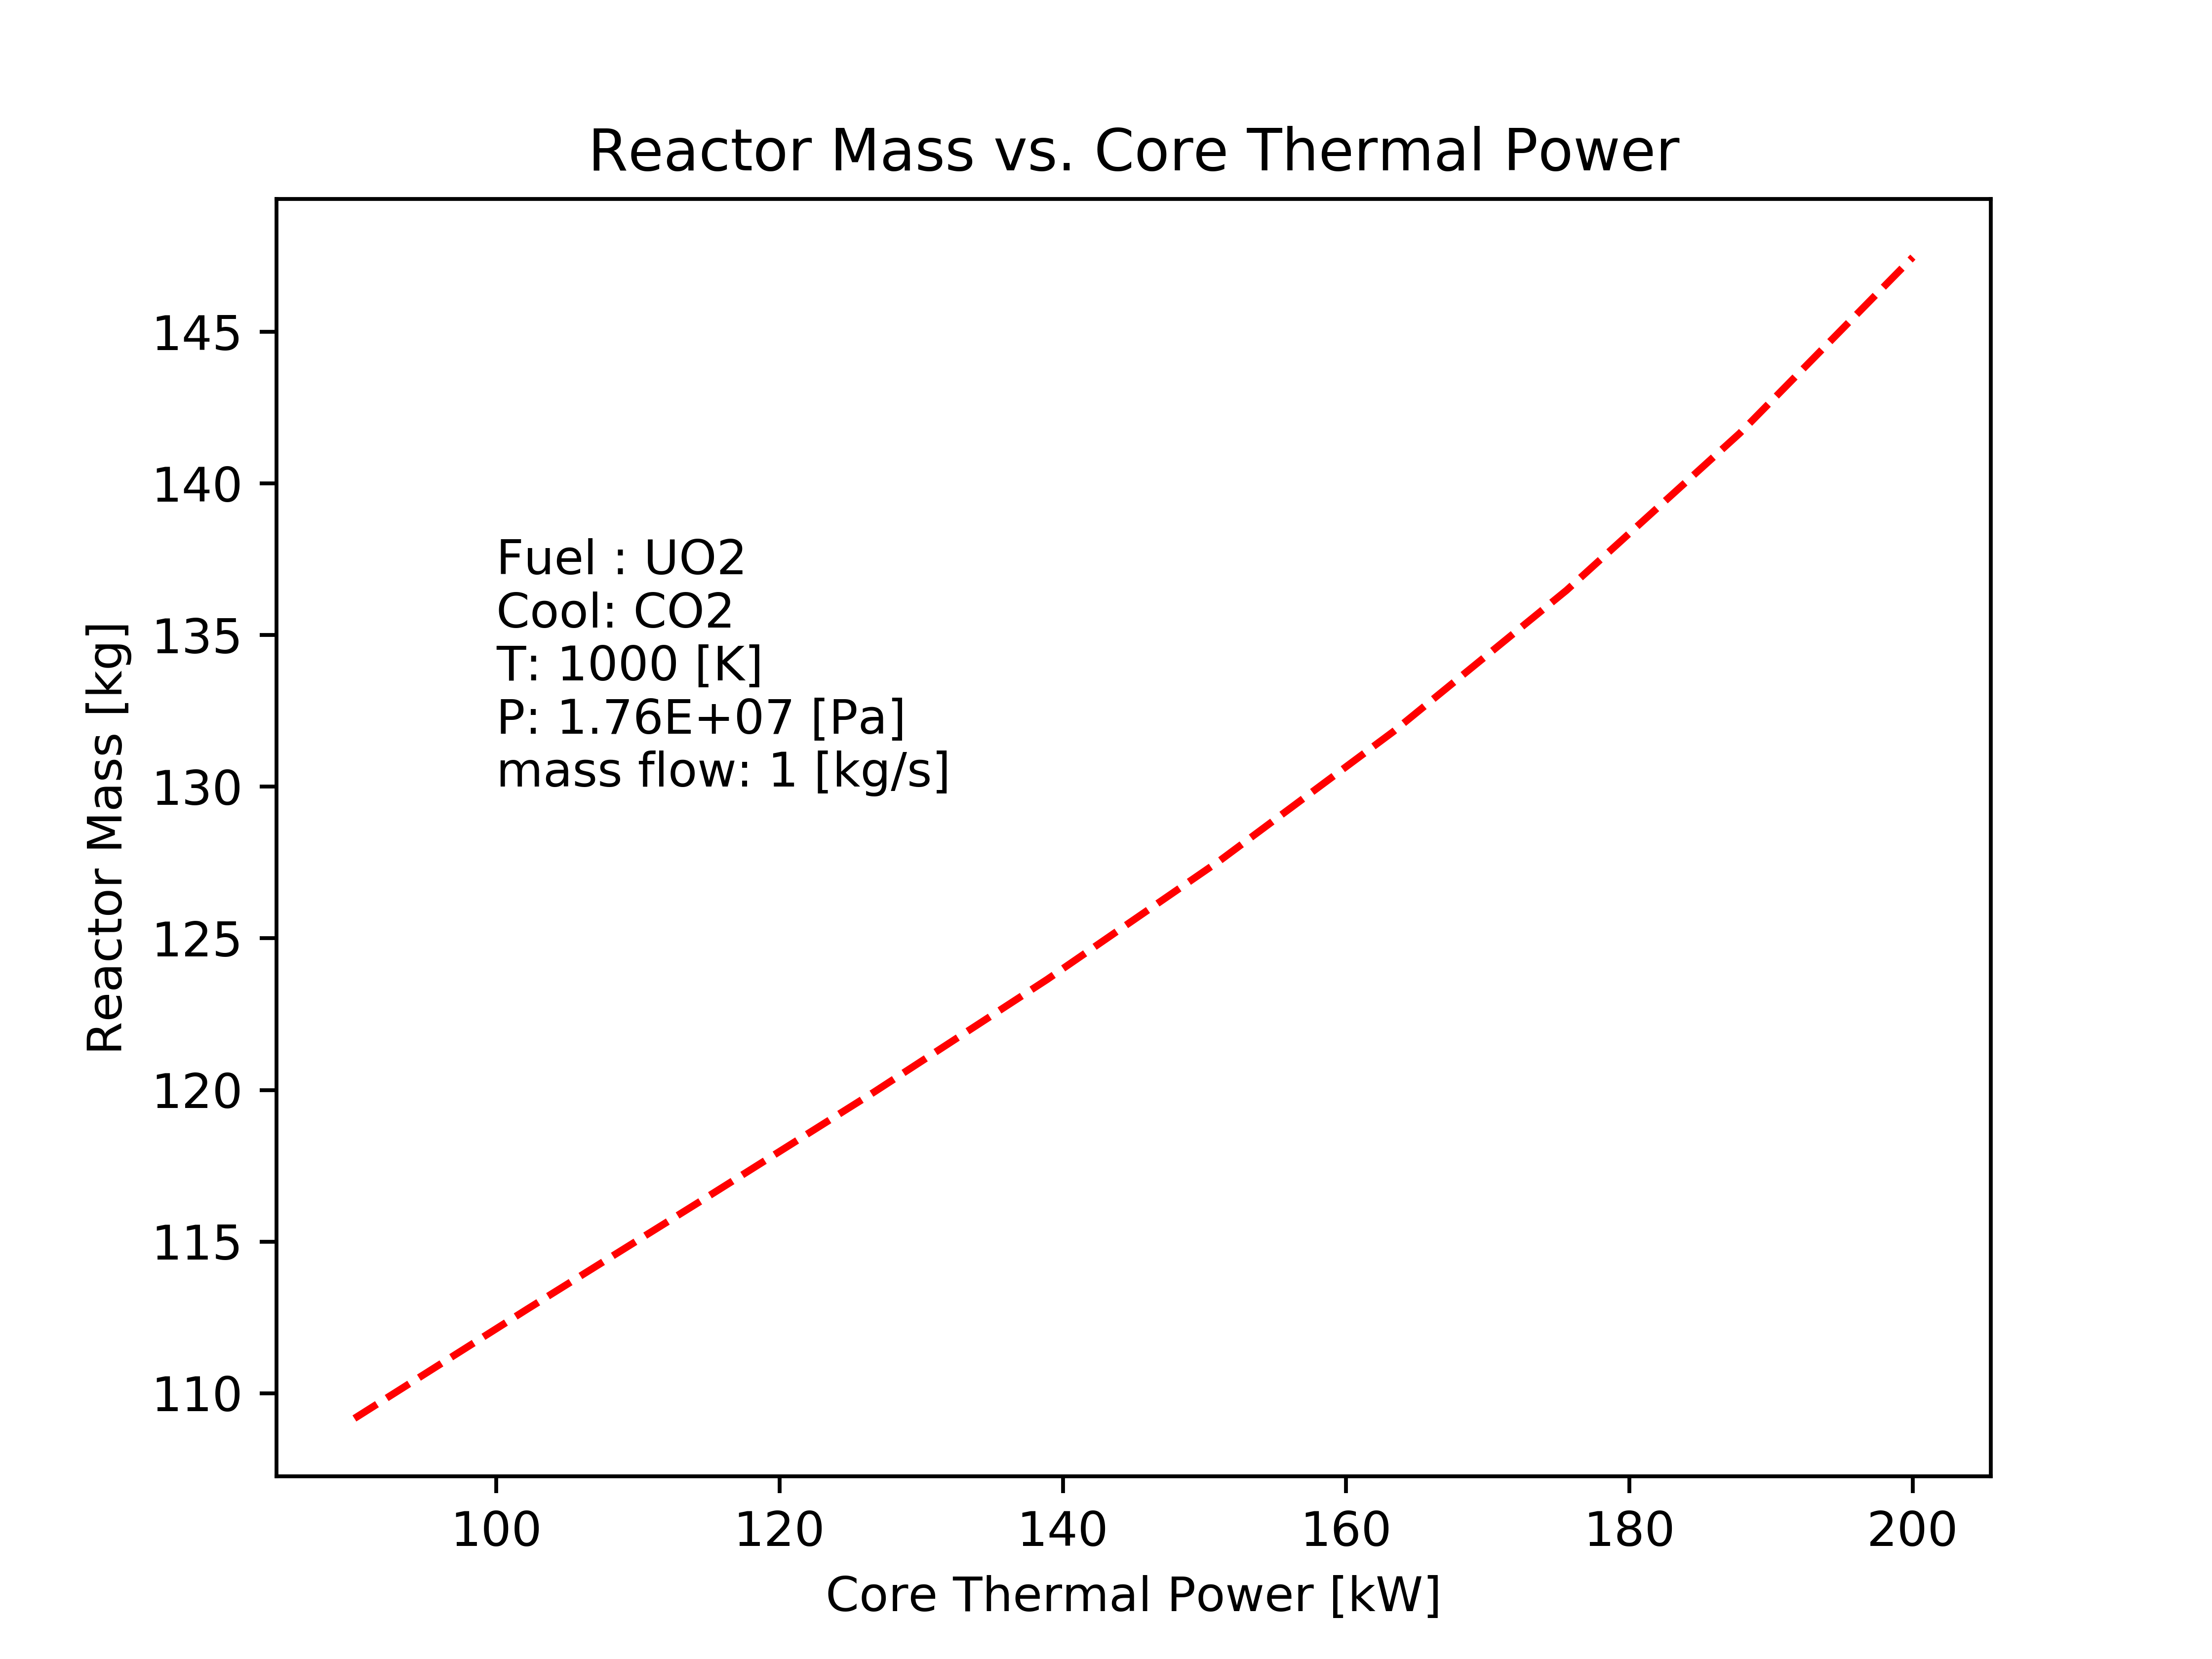
\includegraphics[width=4in]{../images/mass_vs_q_uo2_co2.png}
\caption{Reactor mass power dependence}
\label{fig:mass_vs_q_uo2_co2}
\end{figure}

\section{Overall Cycle Optimization Results}
The reactor mass model was developed to support mass modeling for the entire
electrical power system. Before the reactor model was coupled to the power
cycle, it was interesting to investigate the reactor response to flow
parameters.

\section{Conclusion}
A reactor mass model was developed from thermal hydraulic and reactivity
requirements (discussed in \ref{ch:critical_radius}). The model solved the heat
transfer equations iteratively to return a reactor model that meets the thermal
input requirements of the power cycle. The mass model was demonstrated here for
the \uox-\codiox  reactor configuration. Three other configurations were
considered using UN-\codiox, \uox-\water, and UN-\water. The results of these
configurations, as well as their corresponding reactivtiy models can be found in
Appendix \ref{ch:appendix-a}.


